\chapter{Formation professionnelle continue}

Au-delà de ma formation initiale solide, j'ai suivi tout au long de ma carrière de nombreuses formations continues, témoignant d'un engagement constant dans le développement professionnel \parencite{perrenoud_pratique_reflexive}. Ces formations couvrent à la fois les aspects techniques, pédagogiques et réflexifs, en cohérence avec le profil attendu d'un enseignant du supérieur \parencite{referentiel_meef}.

\section{Certifications professionnelles et formations qualifiantes}

\begin{center}
    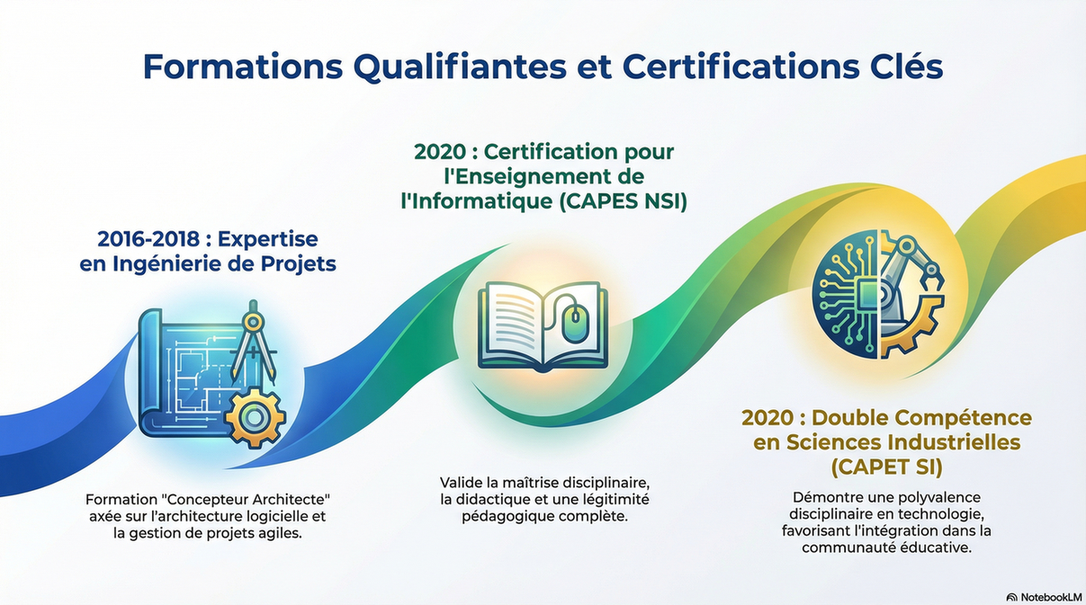
\includegraphics[width=\textwidth]{sources/medias/41.png}
    \\ \vspace{0.5cm} \small \textit{Illustration réalisée avec NotebookLM}
\end{center}

\section{Analyse des formations qualifiantes}

\textbf{Formation Concepteur Architecte (2016-2018)}

Cette formation en contrat de professionnalisation, suivie en parallèle de mon activité chez SopraStéria, illustre ma capacité à concilier responsabilités professionnelles et développement de compétences. Elle préfigure l'approche recherche attendue dans le Master MEEF par :
\begin{itemize}[leftmargin=*]
    \item Méthodologies de conception : transférables à la didactique informatique
    \item Gestion de projets complexes : applicable à l'encadrement d'étudiants
    \item Innovation technologique : nécessaire pour maintenir l'actualité des enseignements
\end{itemize}

\textbf{Double certification CAPES/CAPET (2020)}

L'obtention simultanée de ces deux certifications témoigne d'une reconversion préparée et d'une polyvalence disciplinaire rare. Cette double compétence apporte :
\begin{itemize}[leftmargin=*]
    \item Légitimité pédagogique : certification officielle pour l'enseignement
    \item Vision systémique : approche technologique complémentaire à l'informatique pure
    \item Adaptabilité : capacité à enseigner dans différents contextes
\end{itemize}

\section{Tableau 2 : Formation continue pédagogique (2021-2025)}

\begin{center}
\tiny
\begin{tabular}{|p{2.5cm}|p{1cm}|p{2.5cm}|p{2.5cm}|p{2.5cm}|}
\hline
\textbf{Formation} & \textbf{Année} & \textbf{Programme} & \textbf{Apports} & \textbf{Compétences MEEF} \\
\hline
Évaluation au service de l'élève & 2024/25 & Évaluation formative, différenciation, outils numériques & Modernisation pratiques évaluatives, approche bienveillante & Analyser activité enseignant/élève \\
\hline
Programmation fonctionnelle NSI & 2024/25 & Paradigmes fonctionnels, Lisp/Scheme, applications pédagogiques & Actualisation disciplinaire, nouveaux paradigmes & Didactique, Programmation \\
\hline
Programmation dynamique NSI & 2024/25 & Algorithmes optimisation, mémorisation, applications & Approfondissement algorithmique, techniques optimisation & Algorithmique, Algo avancée \\
\hline
Graphes pour résoudre problèmes NSI & 2024/25 & Théorie graphes, algorithmes parcours, modélisation & Structures données avancées, résolution problèmes complexes & Algorithmique, Structures données \\
\hline
Cartographier des données & 2024/25 & Visualisation données, outils cartographiques, géolocalisation & Data science, visualisation, approche interdisciplinaire & Didactique, Bases données \\
\hline
Formation disciplinaire néotitulaires & 2024/25 & Gestion classe, progression pédagogique, évaluation & Consolidation pratiques, échanges expériences & Praticien réflexif, Se projeter \\
\hline
Journée académique NSI & 2024/25 & Partage expériences, innovations, évolutions programmes & Veille pédagogique, mutualisation pratiques & Praticien réflexif, Recherche \\
\hline
CRCNE auto-évaluation & 2023/24 & Compétences numériques, auto-évaluation, certification & Compétences numériques, réflexivité pratiques & Communauté éducative, Réflexif \\
\hline
Gestes professionnels inclusifs & 2023/24 & Pédagogie inclusive, différenciation, besoins particuliers & Approche inclusive, adaptation diversités & Communauté, Analyser activité \\
\hline
NSI journées thématiques & 2023/24 & Approfondissements disciplinaires, nouvelles ressources & Actualisation connaissances, veille technologique & Didactique, Recherche \\
\hline
SNT Internet et Web & 2022/23 & Protocoles web, sécurité, enjeux sociétaux numérique & Actualisation technique, approche sociétale & Réseaux, Didactique \\
\hline
SNT Micro :bit objets connectés & 2022/23 & Programmation embarquée, IoT, capteurs & Systèmes embarqués, innovation pédagogique & Architecture, Systèmes \\
\hline
Formation transversale T1 & 2022/23 & Gestion classe, relation éducative, communication & Compétences relationnelles, communication & Communauté, Réflexif \\
\hline
NSI échanges de pratiques & 2021-23 & Mutualisation ressources, innovations, retours expérience & Enrichissement pratiques, réseau professionnel & Réflexif, Recherche \\
\hline
\end{tabular}
\end{center}

\section{Analyse des temps forts de la formation continue}

\subsection{Actualisation disciplinaire constante}

Ma participation régulière aux formations NSI (programmation fonctionnelle, dynamique, graphes) illustre un engagement dans l'actualisation disciplinaire conforme aux exigences du Master MEEF. Ces formations correspondent directement aux compétences techniques du référentiel et démontrent ma capacité à maintenir une expertise technique de pointe.

\subsection{Développement des compétences pédagogiques}

Les formations transversales (évaluation, gestes inclusifs, formation des néotitulaires) révèlent une approche réflexive de l'enseignement. Elles correspondent aux compétences transversales et réflexives du Master MEEF et témoignent d'une volonté d'amélioration continue des pratiques pédagogiques.

\subsection{Engagement dans la communauté éducative}

La participation systématique aux journées académiques et échanges de pratiques illustre mon intégration dans la communauté éducative et ma contribution à la mutualisation des savoirs. Cette démarche collaborative correspond parfaitement aux attendus en termes d'intégration dans la communauté éducative.

\section{Correspondances avec le référentiel Master MEEF Informatique}

L'analyse détaillée des correspondances entre ma formation continue et les compétences du Master MEEF Informatique est présentée dans le \textbf{Chapitre 12 - Synthèse de la correspondance}, section \textbf{12.1 Tableau récapitulatif de couverture des blocs de compétences}.

Cette synthèse démontre comment ma démarche de formation continue contribue à l'acquisition et au renforcement des compétences attendues du référentiel RNCP38152.

\section{Impact sur ma pratique professionnelle}

Cette formation continue intensive (plus de 15 jours par an) témoigne d'un engagement professionnel fort et d'une capacité d'adaptation aux évolutions de l'enseignement. Elle illustre parfaitement l'approche attendue dans le Master MEEF : allier expertise disciplinaire, compétences pédagogiques et démarche de recherche.

L'évolution de mes formations, de l'expertise technique pure vers la pédagogie inclusive et l'innovation éducative, révèle une maturation professionnelle cohérente avec ma progression vers l'enseignement supérieur. Cette démarche de formation continue constitue un atout majeur pour contribuer à la formation des futurs enseignants d'informatique dans le cadre du Master MEEF.

\section{Synthèse des acquis de formation continue}

Mon engagement dans la formation continue s'articule autour de trois axes complémentaires :

\begin{enumerate}[leftmargin=*]
    \item \textbf{Actualisation disciplinaire} : Maintien d'une expertise technique de pointe via les formations NSI spécialisées
    \item \textbf{Développement pédagogique} : Amélioration continue des pratiques d'enseignement et d'évaluation
    \item \textbf{Innovation collaborative} : Participation aux groupes de travail nationaux sur l'IA et la forge éducative
\end{enumerate}

Cette triple approche correspond parfaitement aux exigences du Master MEEF Informatique et démontre une posture de praticien-chercheur \parencite{schon_reflective_practitioner} alignée avec les attendus de l'enseignement supérieur.